\section{Introduction}

Large language models (LLMs) have achieved tremendous success in generating answers to user questions~\cite{hadi2023survey,hadi2023large,zhu2023large}. 
% However, they may produce wrong or fictitious responses when lacking specific knowledge to answer the question, e.g., due to outdated training data~\cite{xxx} or missing domain-specific knowledge~\cite{xxx}. 
However, they may produce wrong or fictitious responses when lacking specific knowledge to answer the questions~\cite{wang2023survey,huang2023survey,tonmoy2024comprehensive}, e.g., due to outdated training data or missing domain-specific knowledge. 
In these cases, \textit{retrieval-augmented generation} (RAG)~\cite{lewis2020retrieval} improves answer quality by retrieving contexts related to the user question from an external database and feeding these contexts along with the user question to 
the LLMs for answer generation. Among RAG methods, \textit{graph-based RAG} (a.k.a., GraphRAG) is particularly popular, which uses knowledge graphs as the external databases~\cite{procko2024graph,he2024g,hu2024grag,zhang2024graph}.
This is because knowledge graph is a powerful format of knowledge expression, where the graph nodes represent real-world entities and edges represent the complex relations between the entities~\cite{chen2020review,fensel2020introduction}.         

% their response quality 

% their answer quality degrades when lacking 
% they struggle when lacking specific knowledge to answer   
% The burgeoning advancements in large-scale language models (LLMs) have unveiled several limitations, particularly the prevalence of factual inaccuracies attributable to outdated knowledge bases. To address this issue, Retrieval-Augmented Generation (RAG) models have been proposed, integrating external databases to retrieve up-to-date or domain-specific knowledge during question-answering tasks, thereby enhancing the accuracy and reliability of responses.
% However, it is recognized that knowledge inherently exists in complex graph structures rather than in plain text forms. Motivated by this understanding, researchers have developed Graph RAG, which extends the retrieval mechanism of RAG by incorporating graph processing techniques. Specifically, Graph RAG employs methods such as graph mining and reasoning over knowledge graphs, thereby capturing intricate relationships and hierarchical structures more effectively. This advancement significantly improves the depth and quality of responses, offering a more nuanced understanding of complex knowledge domains.

% {
% \renewcommand{\arraystretch}{2}
% \begin{table*}
%   \caption{Summarization-Based Question Generation}
%   \label{tab:introquestion}
%   \begin{tabular}{ccc}
%     \toprule
%     Technique & Questions \\
%     \midrule
%     Summary Generation & \makecell[l]{
%     1. What therapies can help children like Harry who face family rejection and trauma?\\ 
%     2. How do J.K. Rowling and Rick Riordan differ in their writing styles? \\ 
%     3. How to visualize Mr. Dursley's internal thoughts in storytelling?\\ 
%     4. What quantitative methods can predict box office success from dataset analysis?} \\ 
%     \bottomrule
%   \end{tabular}
% \end{table*}
% }

\begin{figure}[t]
    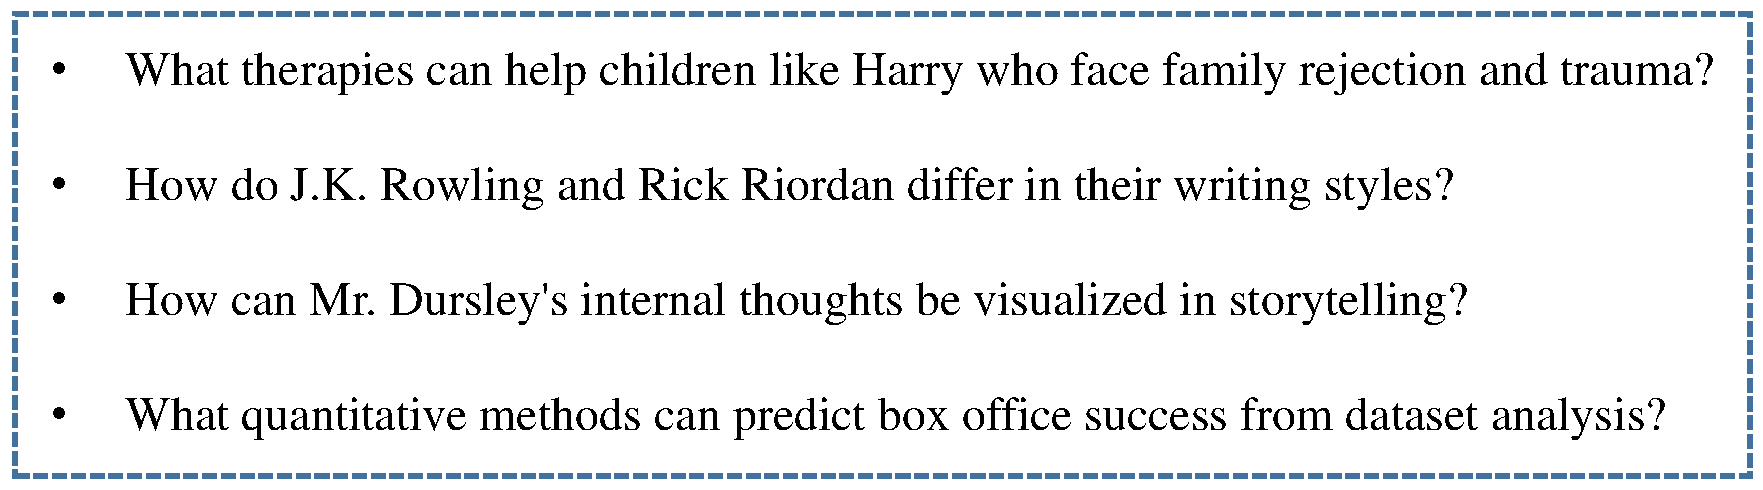
\includegraphics[width=0.5\textwidth]{pictures/introquestion.pdf}
    \centering
    \vspace{-2em}
    \caption{Questions produced for Harry Potter novel by the summary-based method in current evaluation framework.}
    \label{fig:introquestion}
\end{figure}

\begin{figure}[!t]  % 使用 figure 环境，可以添加标题和编号
    \centering  % 图片居中
        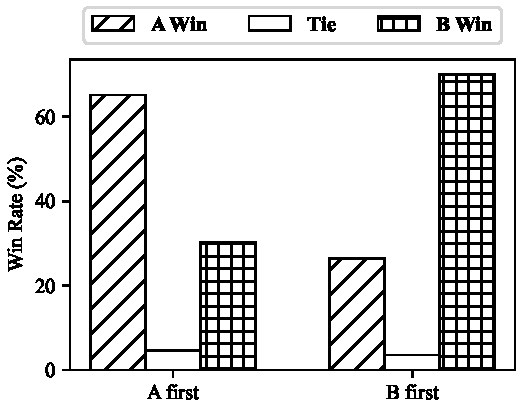
\includegraphics[width=0.6\columnwidth]{pictures/position-bias-result.pdf}  % 插入图片，设置宽度为文本宽度的 50%
    \vspace{-1em}    
    \caption{The position bias for LLM-based answer assessment. We compare the answers generated by LightRAG in 2 runs for the same questions but change the order of the two answers (i.e., `AB' and `BA') when feeding them to the LLM. }  % 添加图片标题
    \label{fig:positionbias}  % 添加标签，用于引用
\end{figure}

Many GraphRAG methods have been proposed, and they mainly differ in how to traverse the knowledge graph and retrieve the related contexts. For instance, Microsoft GraphRAG (called \textit{MGRAG} hereafter to avoid confusion with GraphRAG)~\cite{edge2024local} performs community detection on the knowledge graph and generates text summaries for the communities offline, and during online question answering, it selects the community summaries that have large relevance scores for the user question. LightRAG~\cite{guo2024lightrag} first extracts keywords referring to entities and relations from the user question and then retrieves these entities and relations along with their 1-hop neighbors from the knowledge graph. FastGraphRAG (called \textit{FGRAG} hereafter)~\cite{fastgraphrag2024} first extracts entities from the user question, then retrieves the relevant contents from the knowledge graph according to semantic similarity w.r.t. the extract entities (measured by their vector embeddings), and finally ranks the contents according to their PageRank scores to select the top ones. GraphCot~\cite{jin2024graph} adopts chain of thought~\cite{wei2022chain} and involves an agent (which is an LLM) to determine the node or edge to check in each graph traversal step. Please refer to~\cite{procko2024graph,han2024retrieval} for a survey of GraphRAG methods. 

%\xiao{given the former paragraph, we may not need to introduce GraphRAG methods in the paper}

Since human inspection is expensive, GraphRAG methods are usually evaluated with LLMs for their answer quality. In particular, an evaluation framework consists of two parts, i.e., \textit{question generation} and  \textit{answer assessment}. For question generation,  MGRAG~\cite{edge2024local} and LightRAG~\cite{guo2024lightrag} extract the head and tail of each passage in the dataset as the passage summary, and the summaries of all passages are aggregated as dataset summaries, which are fed to an LLM for question generation.
For answer assessment, an LLM is requested to compare the answers produced by two RAG methods for the same question, in aspects such as \textit{Comprehensiveness}, \textit{Diversity}, \textit{Empowerment}, and \textit{Directness}, e.g., using a prompt like `\textit{Please choose the better answer from A and B for question Q in term of $\cdots$}', where $A$ and $B$ are the answers produced by two RAG methods. An overall winner is determined based on the separate winners of each aspect, and the win rate of a method is the percentage of questions it wins.

% \xiao{we are discussing the question generation method and answer assessment of which paper? check the details}


% Although research on GraphRAG is progressing rapidly, the development of its evaluation system remains relatively underexplored. The evaluation of GraphRAG is primarily divided into two parts: question generation and answer quality assessment.
% In the question generation part, some studies utilize existing datasets with pre-defined questions, while others generate questions based on the datasets themselves. During the question generation stage, a summarization-based approach is commonly adopted. Specifically, the head and tail of each passage in the dataset are spliced together to form a summary of that passage. These summaries are then aggregated to create a summary of the entire dataset, which is subsequently fed into a large language model (LLM) to generate questions.
% In the answer quality evaluation phase, methods that use datasets with pre-defined questions compare the generated answers with the ground truth answers. In contrast, other methods employ the LLM as a judge. Specifically, they design specific criteria to evaluate answer quality and feed the generated answers into the LLM, asking it to assess which answer is better based on these criteria.

%make it difficult to assess the performance gains of GraphRAG methods
We observe that current method for GraphRAG evaluation has two critical flaws that hinder scientific performance assessment. 
\squishlist
\item \textit{Unrelated questions}. Figure~\ref{fig:introquestion} lists some example questions generated using the \textit{summary-based method} in existing evaluations for the Harry Potter novel. It is obvious that these questions are overly broad and vague. Moreover, they are not (closely) related to the Harry Potter story. This is because the LLM is only provided with vague summaries of the passages in the dataset for question generation, and as a result, the questions do not involve the fine-grained details of the passages. However, GraphRAG is expected to retrieve fine-grained details from knowledge graphs to supplement the LLMs for answer generation, and such ability can not be evaluated using the questions in Figure~\ref{fig:introquestion}.   


\item \textit{Evaluation biases}. We find that the current evaluation protocol has three biases that hinder scientific performance assessment, i.e., \textit{position bias}, \textit{length bias}, and \textit{trial bias}. In particular, position bias means that simply changing the positions of the two compared answers in the evaluation prompt has a significant impact on the evaluation result. We show such an example in Figure~\ref{fig:positionbias}, where the positions of two answers `\textit{A}' and `\textit{B}' are changed from `\textit{AB}' to `\textit{BA}'. Since we compare the same GraphRAG method (i.e., LightRAG) with itself, the result should be a tie. However, LLMs favor the answer that comes in the front, and the win rates can differ by over 30\%. Similarly, length bias means that LLMs favor longer answers, and trial bias means that an LLM can produce different results when evaluating two answers multiple times.     

\squishend



% We conducted experiments and analyses on current approaches to summarization-based question generation as well as answer quality evaluation. Our findings revealed that there are significant issues with both \textbf{question generation} and \textbf{answer quality evaluation}. Traditional question generation based on generalization often struggles to accurately capture the essence of a dataset. As a result, it resorts to simply splicing the beginning and the end of a paragraph to serve as a summary. This approach places high demands on the structure of the paragraph and is particularly ineffective for narrative-style paragraphs, such as those found in stories. In such cases, the generated summary may fail to accurately represent the content, leading to overly broad or even unanswerable questions based on the dataset. For example, using the Harry Potter dataset, we list the questions generated based on this summarization method in Table ~\ref{fig:introquestion}. It is evident that most of these questions are only loosely related to the story of Harry Potter and are overly broad and vague.
% In the evaluation of answer quality, we have identified three biases in the current method of using LLMs as judges: position bias, length bias, and trial bias. Specifically, LLMs tend to favor the first answer they receive, prefer longer answers, and exhibit instability in their evaluations. When the quality of answers is similar, minor variations in evaluation conditions can lead to inconsistent results.





To tackle the flaws of the current GraphRAG evaluation, we design an unbiased evaluation framework with two innovations.

\squishlist
\item \textit{Graph-text-ground question generation}. To ensure that the questions correspond to fine-grained details of the dataset, we use the knowledge graph derived from the dataset to guide question generation. In particular, to generate a question, we first sample a structure from the knowledge graph (i.e., node, edge, or subgraph) and then feed the structure and its related contexts to an LLM for question generation. This graph-text-grounded method allows us to configure the type of the generated question, i.e., related to a node, a relation, or a subgraph. We show with concrete examples that our questions are much more related to the dataset than those generated using the summary-based method.



\item \textit{Unbiased evaluation procedure}. We design a comprehensive evaluation procedure to eliminate the aforementioned biases. In particular, the position bias is handled by evaluating both `\textit{AB}' and `\textit{BA}', and a tie is declared if the overall scores obtained by the two answers are the same. For the length bias, we first let two methods generate their answers and then perform answer alignment to align the shorter answer with the longer one in length. For the trial bias, we conduct multiple rounds of evaluation with each round covering all the questions and report the statistics of the rounds (e.g., median, and the percentiles).  

\squishend










We applied our unbiased evaluation framework to compare 3 representative GraphRAG methods, i.e., MGRAG, LightRAG, and FGRAG, and directly retrieving the text chunks without knowledge graph (called NaiveRAG)~\cite{gao2023retrieval} is included as a baseline. The results show that the significant performance gains reported by existing research may be caused by the biases, and after eliminating the biases, the  
performance gains become much more moderate or even vanish. Figure~\ref{fig:introbias} provides such an example, where LightRAG originally outperforms NaiveRAG with a win rate of 72\% vs. 28\% but NaiveRAG slightly outperforms LightRAG after eliminating the biases. This is because LightRAG usually generates longer answers than NaiveRAG, and the original evaluation always places its answer before NaiveRAG. We do observe that FGRAG outperforms the others but again the performance gains are moderate, i.e., below 10\% in win rate expect when compared with LightRAG. 

%\zqm{performance gains over NaiveRAG?}




% We applied our graph-grounded question generation mechanism to create multi-level questions for several datasets and evaluated the answer quality of responses generated by popular Graph RAG models using our proposed unbiased evaluation system. We propose a metric called the Actual Gain Rate (AGR), which is used in conjunction with the calculation of the actual gain in performance of the RAG model. Our findings reveal that the test results are not entirely consistent with those reported in their respective papers. Specifically, Fast Graph RAG performs the best under our evaluation framework, but its lead-over Graph RAG is marginal, and the performance gap between Light RAG and Naive RAG is not particularly significant. This raises questions about whether current advancements in the field of Graph RAG truly represent substantial improvements over traditional methods.
% To further investigate, we conducted additional experiments on token consumption and query time. These experiments confirmed that Fast Graph RAG achieves excellent results with fewer tokens and faster query speeds. We hope that our work encourages scholars to re-examine the progress in the Graph RAG field and provides an objective and fair evaluation system for future research. Additionally, our findings offer theoretical support for enterprises in selecting appropriate models for their needs.

\begin{figure}[!t]  % 使用 figure 环境，可以添加标题和编号
	\centering  % 图片居中
	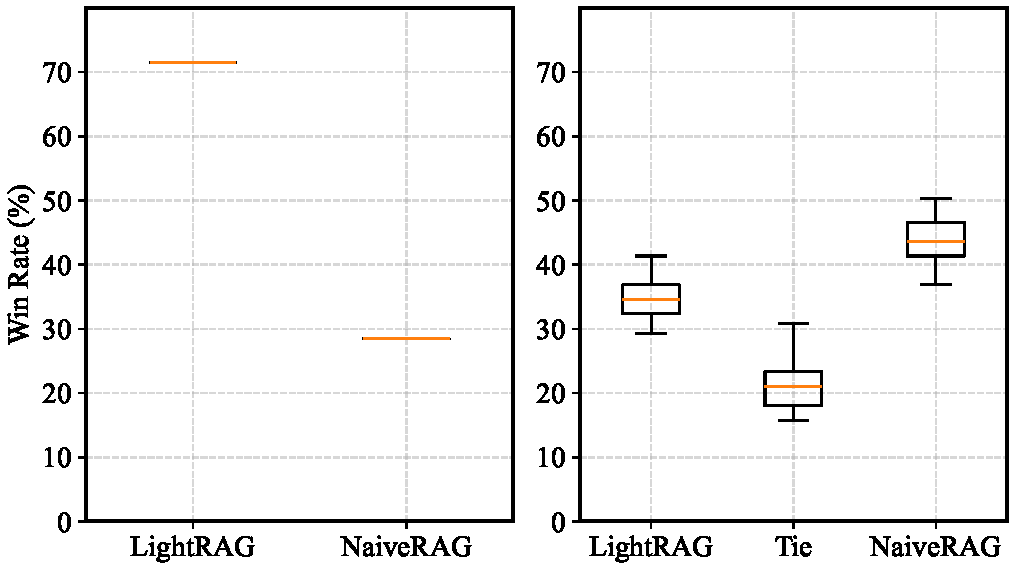
\includegraphics[width=0.8\columnwidth]{pictures/introbias.pdf} % 插入图片，设置宽度为文本宽度的 50%
	%\vspace{-0.8em}
	\caption{The evaluation results using the existing method (left) and our unbiased framework (right). Note that existing method does not allow ties. In the box plot (right), the red line is the median, and the lower and upper box boundaries are the 25th and 75th percentiles, respectively.}  % 添加图片标题
	\label{fig:introbias}  % 添加标签，用于引用
\end{figure}

To summarize, we make the following contributions:

\squishlist
\item We observe that the current method for GraphRAG performance evaluation has critical flaws, i.e., \textit{unrelated questions} and\textit{ evaluation biases}, that may lead to biased or wrong conclusions.


\item We design a new evaluation framework for GraphRAG, which tackles the flaws of the existing method with \textit{graph-text-ground question generation} and \textit{unbiased evaluation procedure}. 

\item We compare representative GraphRAG methods using our evaluation framework. The results suggest that existing GraphRAG researches are overly optimistic about their performance gains.    

\squishend

We note that our evaluation framework may still be far from perfect. However, given the rapid advances of GraphRAG methods, our work does show that a scientific evaluation framework for their performance is lacking, and without it, we cannot assess whether GraphRAG researches make real progress. We hope that our work can inspire more work on performance evaluation.  


% \textbf{1. We propose a graph-grounded question generation mechanism}, which utilizes the graph structure knowledge base for graph mining operations and can dynamically generate multi-level problems for different datasets.

% \textbf{2. We propose an unbiased evaluation system that can evaluate the Graph RAG answering ability in the case of no ground truth.} We utilize the ideas of answer alignment operation, position exchange, and median in terms of probability to overcome multiple biases. Therefore, constructing a relatively objective evaluation system for Graph RAG.

% \textbf{3. Evaluating Several existing representative Graph RAGs.} Their evaluation results under our evaluation system were obtained, and the results were analyzed from a theoretical point of view. Thus, encouraging scholars to re-examine the progress in the Graph RAG field.